\chapter{Praktische Evaluation}

\section{Testumgebung}
Die folgenden Experimente wurden auf mithilfe einer AMD EPYC 7763 64-Core CPU mit 16 nutzbaren Hardwarethreads und 64GB Arbeitsspeicher durchgeführt. Das System
verwendet Ubuntu 24.04 als Betriebssystem und GCC in der Version 13.2.0 als Compiler. Die Ausführung der Algorithmen mit einer spezifischen Anzahl von Threads wurde
softwareseitig über OpenMP-Instruktionen realisiert. 

\section{Implementierung}

\subsection{Klassenstruktur}

\subsection{Code}
Die konkrete Implementierung erfolgte in der Programmiersprache C++ im C++20 - Standard und dem Build - System CMake in der Version 3.28. Die Parallelisierung wurde
über Präprozessor - Instruktionen von OpenMP realisiert.

\section{Messung}

\subsection{Eingabedaten}
Die folgenden Algorithmend wurden auf verschiedenen Dateien aus dem Pizza \& Chili-Corpus getestet. Die verwendeten Dateien decken verschiedene Kontexte und damit
Kompressionspotentiale ab.
\begin{figure}
    \centering
    \caption{Auflistung der verwendeten Eingabedaten}
    \label{inputdata}
    \begin{tabular}{|c|c|c|c|c|}
        \hline
        \textbf{Datei} & \textbf{Größe} & \textbf{Alphabet} & \textbf{Beschreibung} \\
        \hline
        \texttt{dna} & 100MB & 4 & DNA-Sequenzen \\
        \hline
        \texttt{english} & 100MB & 256 & Englische Texte \\
        \hline
        \texttt{proteins} & 100MB & 20 & Proteinsequenzen \\
        \hline
        \texttt{sources} & 100MB & 256 & Quellcode \\
        \hline
        \texttt{xml} & 100MB & 256 & XML-Dateien \\
        \hline
    \end{tabular}
\end{figure}
In der Tabelle \ref{inputdata} sind die verwendeten Dateien aufgelistet. Die Größe der Dateien wurde auf 100MB beschränkt, um einen angemessenen Rahmen für die 
Laufzeitmessung zu erhalten.

\subsection{Messgrößen}

\subsubsection{Laufzeit}
Die Laufzeit der Algorithmen wurde innerhalb der Ausführung gemessen. Dabei wird die Zeitmessung nach dem Laden der Eingabedatei gestartet und mit dem vollständigen
Auffüllen der Faktorfolge beendet. Damit wird das Einlesen der Eingabe und eine eventuelle Kodierung der Ausgabe nicht in die Laufzeitmessung einbezogen. Diese Strategie
hat ihren Hintergrund in der Tatsache, dass die konkrete Ausprägung des Eingabe- und Ausgabestroms keine Aussagekraft über die Qualität der Kompression hat.

\subsubsection{Speicher}
Der Speicherverbrauch der Algorithmen wurde auch intern mithilfe einer externen Bibliothek gemessen. Dabei wurden Speicherallokationen auf dem Heap überwacht und 
gemessen. Im Rahmen dieser Arbeit wurde die Spitze des allokierten Speichers im Zeitraum nach dem Einlesen der Eingabedatei und nach dem vollständigen Auffüllen der
Faktorfolge gemessen.

\subsection{Messwerte}

\subsubsection{Laufzeiten}
\begin{figure}
    \centering
    \caption{Laufzeit der Algorithmen auf Präfixen verschiedener Größen der Datei Proteins}
    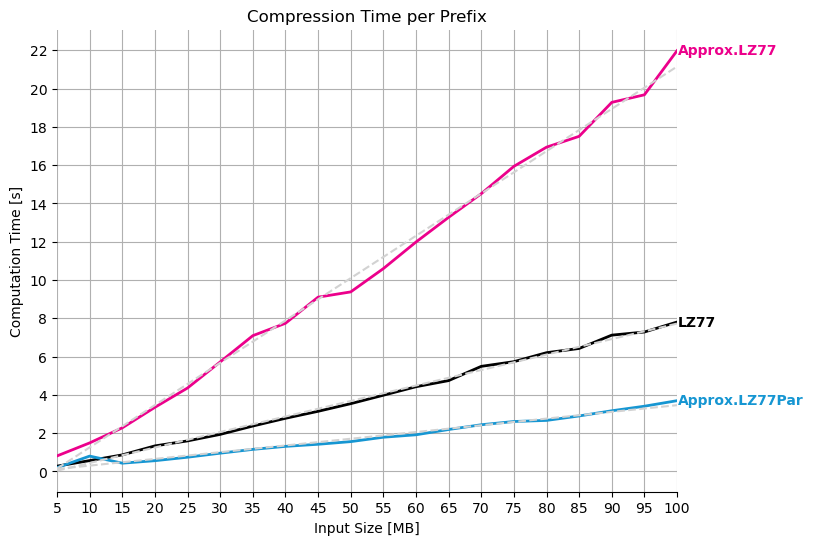
\includegraphics[scale=0.6]{Images/progressive.png}
    \end{figure}
    
\begin{figure}
    \centering
    \caption{Laufzeit der parallelen Approximation von LZ77 mit verschiedenen Anzahlen von Threads}
    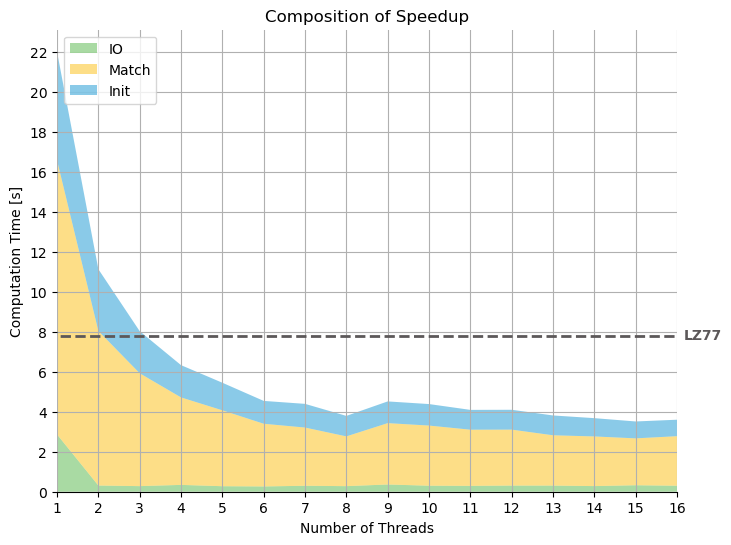
\includegraphics[scale=0.6]{Images/progressive_speedup_stack.png}
\end{figure}

\subsubsection{Speicherverbrauch}

\subsubsection{FR und CR*}

\section{Auswertung}
\subsection{LZ77}
\subsection{Approx. LZ77}
\subsection{Approx. LZ77Par}